% !TEX program = xelatex
% ============================================================
%  第一届天津市五校数学建模联赛 A 题 论文
%  低空经济背景下的多无人机协同巡检路径优化问题
%  编译：xelatex main.tex
% ============================================================
\documentclass[12pt,a4paper]{ctexart}

% ---------- 页面与几何 ----------
\usepackage[a4paper,top=2.5cm,bottom=2.5cm,left=2.5cm,right=2.5cm]{geometry}

% ---------- 数学 ----------
\usepackage{amsmath,amssymb,amsthm}

% ---------- 表格 ----------
\usepackage{booktabs,multirow,array}

% ---------- 图片 ----------
\usepackage{graphicx}
\usepackage{float}
\usepackage{subcaption}
\usepackage{tikz}
\captionsetup{font=small,labelfont=bf}

% ---------- 页眉页脚 ----------
\usepackage{fancyhdr}

% ---------- 代码 ----------
\usepackage{listings}
\usepackage{xcolor}
\definecolor{codegreen}{rgb}{0.1,0.55,0.1}
\definecolor{codeblue}{rgb}{0.1,0.25,0.65}
\definecolor{codeorange}{rgb}{0.85,0.4,0.1}
\lstset{
  basicstyle=\ttfamily\footnotesize,
  breaklines=true,
  breakatwhitespace=false,
  postbreak=\mbox{\textcolor{gray}{$\hookrightarrow$}\space},
  columns=fullflexible,
  keepspaces=true,
  showstringspaces=false,
  frame=single,
  framerule=0.4pt,
  numbers=left,
  numberstyle=\tiny\color{gray},
  stepnumber=1,
  language=Python,
  commentstyle=\color{codegreen},
  keywordstyle=\color{codeblue},
  stringstyle=\color{codeorange},
  extendedchars=true,
  captionpos=b
}

% ---------- 超链接 ----------
\usepackage[bookmarksnumbered=true,colorlinks=true,linkcolor=blue,citecolor=blue,urlcolor=blue]{hyperref}

% ---------- 列表 ----------
\usepackage{enumitem}
\setlist{nosep}

% ============================================================
%  队伍控制号（请替换为实际队伍控制号）
% ============================================================
\newcommand{\teamno}{TJMML2026073}

% ---------- 页眉页脚样式 ----------
\fancypagestyle{front}{%
  \fancyhf{}
  \fancyfoot[C]{\thepage}
  \renewcommand{\headrulewidth}{0pt}
}
\fancypagestyle{body}{%
  \fancyhf{}
  \fancyhead[R]{\zihao{-5} 队伍控制号：\teamno}
  \fancyfoot[C]{\thepage}
  \renewcommand{\headrulewidth}{0.4pt}
}

\setlength{\parskip}{3pt plus 1pt}

\begin{document}

% ============================================================
%  第 1 页：摘要页（含标题与关键词，不超一页）
% ============================================================
\pagestyle{front}
\thispagestyle{front}

\begin{center}
  {\zihao{-2}\bfseries 低空经济背景下的多无人机协同巡检路径优化问题}\\[6pt]
  {\zihao{-3} 摘\quad 要}
\end{center}

\noindent
本文针对低空经济背景下多无人机协同巡检的路径规划问题，围绕\textbf{任务分配}、\textbf{路径优化}、\textbf{负载均衡}与\textbf{临时禁飞区规避}四个方面，建立了最小最大多旅行商问题（min--max mTSP）模型，并设计了高效的元启发式求解算法，完成了对全部四个算例的求解。

针对\textbf{问题一}，将不同巡检等级（I 级 3 次、II 级 2 次、III 级 1 次）的巡检点按巡检次数要求复制扩展为巡检作业集合，以各无人机工作时间最大值最小化为目标建立 min--max mTSP 模型。推导了无人机数量的理论下界
$N\ge \lceil (S+T_{\mathrm{MST}})/9\rceil$
（其中 $S$ 为总服务时长，$T_{\mathrm{MST}}$ 为含基地的最小生成树飞行时长），并以下界为起点逐一验证，确定四个算例的最小无人机数 $N_{\min}$ 分别为 \textbf{4、2、4、4}，对应最长工作时间均控制在 9 h 时限以内。

针对\textbf{问题二}，在问题一基础上引入字典序目标 $(\max_j T_j,\ \delta)$，在保证总体完成时间不增加的前提下最小化无人机间负载差 $\delta=|T_{\max}-T_{\min}|$，通过带字典序接受准则的局部搜索得到均衡调度方案，四个算例的负载差 $\delta$ 分别降至 \textbf{0.074、0.057、0.067、0.026} h。

针对\textbf{问题三}，建立了圆形时间窗禁飞区的绕行几何模型（双切线$+$圆弧最短绕行路径）与巡检点等待策略，提出\textbf{``有效距离矩阵不动点迭代 $+$ 时间感知贪心排序 $+$ 2-opt''}的求解框架，在满足飞行管制约束的同时兼顾总完成时间与负载均衡。四个算例问题三的最长工作时间分别为 8.18、9.38、8.80、7.92 h，负载差低至 0.003--0.138 h。

求解结果验证了本文模型与算法的合理性与有效性，可为城市低空多无人机协同巡检的规模化部署提供可复用的决策支持。

\vspace{8pt}
\noindent\textbf{关键词：}多无人机协同巡检；最小最大车辆路径问题；迭代局部搜索；时间窗禁飞区；负载均衡

\clearpage

% ============================================================
%  第 2 页：目录页
% ============================================================
\pagestyle{front}
\thispagestyle{front}
\setcounter{tocdepth}{1}
\tableofcontents
\thispagestyle{front}
\clearpage

% ============================================================
%  第 3 页起：正文（右上角注明队伍控制号）
% ============================================================
\pagestyle{body}

\section{问题重述}

\subsection{问题背景}

随着低空经济的快速发展，无人机凭借机动灵活、部署便捷、运行成本低等优势，已广泛应用于电力巡检、通信保障、交通监测、河道巡查、森林防火等领域。某市计划建设覆盖全域的智能无人机巡检系统，对输电线路、变电站、通信基站、桥梁、交通枢纽及重点公共设施开展周期性巡检。所有无人机由同一低空飞行基地统一调度，按预先规划的路径执行任务并在完成后返回基地。由于巡检区域广、目标多、规模大，如何合理分配任务并规划路径，是提升巡检效率、降低运行成本的关键。

实际中，不同设施的重要程度与风险等级不同：普通目标一次巡检即可，而变电站、机场导航设施、通信核心节点、跨江桥梁等关键设施需从不同方向、高度或时间多次巡检以降低遮挡、光照与设备误差的影响。因此巡检任务按重要程度划分为 I、II、III 三个巡检等级，分别对应 \textbf{3、2、1} 次巡检。

\subsection{问题的提出}

已知：所有无人机为同型号工业级多旋翼无人机，平均巡航速度 $55\ \mathrm{km/h}$（忽略起降时间），每完成一个巡检点一次巡检作业平均耗时 5 min；飞行基地坐标为 $(0,0)$；附件 1 给出各巡检点坐标与巡检等级（坐标单位 $1$ 对应实际距离 $100\ \mathrm{m}$）；所有无人机同时起飞，仅完成自身全部任务后返回基地，不考虑续航限制。需解决以下三个问题：

\textbf{问题 1}：若要求 9 小时内完成全部巡检任务，需投入 $N$ 架无人机，求 $N$ 的理论最小值 $N_{\min}$；并在采用 $N_{\min}$ 架无人机条件下设计任务分配与路径方案，使总体完成时间尽可能短。

\textbf{问题 2}：在问题一方案基础上，兼顾各无人机工作负载均衡，使各机工作时长尽可能接近，同时保证总体完成时间尽可能短。

\textbf{问题 3}：考虑圆形临时飞行管制区（禁飞区），无人机每天 8:00 开始执行任务，管制区出现时间、圆心与半径见附件 2。在满足巡检需求与管制要求前提下，设计路径方案使总完成时间尽可能短，并提升负载均衡性。

\section{问题分析}

\textbf{问题一}本质上是带\textbf{复制巡检点（split delivery）}的多旅行商问题：同一巡检点按等级可被同一架或不同架无人机多次访问，每次访问消耗 5 min 服务时间。由于目标是最小化最长无人机工作时间，属\textbf{最小最大（min--max）}优化，即平衡型多旅行商问题。$N_{\min}$ 的确定需要先在理论上给出无人机数量的\textbf{下界}，再以计算方式验证下界处是否可行。

\textbf{问题二}在问题一基础上引入\textbf{负载均衡}作为第二目标，属于\textbf{双目标（字典序）}优化：第一优先级仍是最小化最长工作时间 $T_{\max}$，第二优先级是最小化负载差 $\delta=T_{\max}-T_{\min}$，通过字典序搜索实现。

\textbf{问题三}的难点在于\textbf{时间相关}的路径规划：某航段是否需绕行取决于无人机\textbf{到达该航段时刻}禁飞区是否处于活动状态，路径决策与时间耦合，静态距离矩阵不再适用。我们采用``空间聚类分配 $+$ 绕行几何 $+$ 有效距离矩阵不动点迭代 $+$ 时间感知调度''的分层求解框架。

\section{模型假设与符号说明}

\subsection{模型假设}

\begin{enumerate}
  \item 所有无人机同型号、同巡航速度（55 km/h），忽略起飞、降落与加减速耗时；
  \item 无人机巡航路径为两巡检点（或基地）之间的直线段（受禁飞区约束时沿绕行折线段）；
  \item 每完成一次巡检作业耗时固定为 5 min，与巡检等级无关；同一巡检点多次巡检按多次作业计；
  \item 不考虑无人机续航、充电与空域冲突，多架无人机可同时在同一区域飞行；
  \item 禁飞区为圆形，仅在给定时间窗内禁止进入/穿越，其余时段可自由通行；
  \item 无人机 8:00 同时从基地出发，问题一、二以相对时刻 0 计时，问题三以绝对时刻计时。
\end{enumerate}

\subsection{符号说明}

\begin{table}[H]
  \centering
  \caption{主要符号说明}
  \label{tab:symbol}
  \small
  \begin{tabular}{@{}ll@{}}
    \toprule
    符号 & 含义 \\
    \midrule
    $n$ & 巡检点数量（不含基地）\\
    $V=\{1,\dots,n\}$，$0$ & 巡检点集合与基地 \\
    $l_i$ & 巡检点 $i$ 的巡检等级，$l_i\in\{\mathrm{I,II,III}\}$ \\
    $k_i$ & 巡检点 $i$ 要求的巡检次数，$k_i\in\{3,2,1\}$ \\
    $M=\sum_i k_i$ & 总巡检作业次数（visit 数）\\
    $W=\{1,\dots,M\}$ & 复制扩展后的巡检作业集合 \\
    $s=5/60$ h & 单次巡检作业服务时长 \\
    $d_{ab}$ & 点 $a$ 到点 $b$ 的直线飞行时间（h）\\
    $N$ & 投入的无人机数量 \\
    $T_r$ & 第 $r$ 架无人机的工作时长（h）\\
    $T_{\max}=\max_r T_r$ & 系统总体完成时间（h）\\
    $T_{\min}=\min_r T_r$ & 单架无人机最短工作时间（h）\\
    $\delta=T_{\max}-T_{\min}$ & 负载均衡差（h）\\
    $T_{\mathrm{MST}}$ & 基地$\cup V$ 最小生成树的飞行时长下界（h）\\
    $(c_z,r_z)$，$[t_z^0,t_z^1]$ & 禁飞区 $z$ 的圆心、半径与活动时间窗 \\
    \bottomrule
  \end{tabular}
\end{table}

\section{问题一：最小完成时间的多机协同巡检模型}

\subsection{时间计算与数据预处理}

记巡检点 $i$ 的坐标为 $(x_i,y_i)$（单位为 $100\ \mathrm{m}$），基地坐标为 $(0,0)$。任意两点 $a,b$ 间的直线飞行时间为
\begin{equation}
  d_{ab}=\frac{0.1\cdot\sqrt{(x_a-x_b)^2+(y_a-y_b)^2}}{55}\quad(\mathrm{h}).
  \label{eq:dist}
\end{equation}
单次巡检作业服务时长 $s=5/60\ \mathrm{h}$。将每个巡检点 $i$ 按其巡检次数 $k_i$ 复制为 $k_i$ 个作业，得到作业集合 $W$，$|W|=M$。记作业 $j\in W$ 所在的巡检点为 $p(j)$。

\subsection{min--max mTSP 模型}

引入 0--1 决策变量：$y_{abr}=1$ 表示第 $r$ 架无人机在路径中由点 $a$ 直接飞向点 $b$；$x_{jr}=1$ 表示作业 $j$ 分配给第 $r$ 架无人机。则问题一可建模为
\begin{equation}
  \min\ T_{\max}=\max_{r=1,\dots,N} T_r,
  \label{eq:p1obj}
\end{equation}
其中第 $r$ 架无人机的工作时长为
\begin{equation}
  T_r=\sum_{a\in\{0\}\cup V}\sum_{b\in\{0\}\cup V} y_{abr}\,d_{ab}\ +\ s\sum_{j\in W} x_{jr},
  \label{eq:tr}
\end{equation}
约束条件为：
\begin{align}
  & \sum_{r=1}^{N} x_{jr}=1,\quad \forall j\in W, \label{eq:assign}\\
  & \sum_{b} y_{0br}=\sum_{b} y_{b0r}=1,\quad r=1,\dots,N, \label{eq:degree0}\\
  & \sum_{a} y_{apr} - \sum_{b} y_{pbr}=0,\quad \forall p\in V,\ \forall r, \label{eq:flow}\\
  & \sum_{a\in S}\sum_{b\in S} y_{abr}\le |S|-1,\quad \forall S\subset V,\ |S|\ge 2,\ \forall r, \label{eq:subtour}\\
  & \sum_{b} y_{p(j),b,r} = x_{jr}\ (\text{访问约束}),\quad y_{abr},x_{jr}\in\{0,1\}.
\end{align}
式 \eqref{eq:assign} 保证每个作业恰好被一架无人机完成；式 \eqref{eq:degree0}--\eqref{eq:flow} 保证每架无人机从基地出发、回到基地且路径连通；式 \eqref{eq:subtour} 为子回路消除约束。该模型为 NP--难问题，需设计启发式算法求解。

\subsection{无人机数量 $N_{\min}$ 的理论下界}

设总服务时长
\begin{equation}
  S=M\cdot s=\frac{M}{12}\ (\mathrm{h}),
\end{equation}
总飞行时长的下界为覆盖基地与全部巡检点的\textbf{最小生成树（MST）}权重 $T_{\mathrm{MST}}$。理由如下：任意可行方案中，每架无人机的路径均从基地出发并返回，故所有路径的并集构成基地$\cup V$ 上的一个连通子图，其总边权（飞行时长）必不小于 MST 权重 $T_{\mathrm{MST}}$；而总服务时长固定为 $S$。于是全体无人机总工作时长满足
\begin{equation}
  \sum_{r=1}^{N} T_r = \text{总飞行时长} + S \ge T_{\mathrm{MST}} + S.
\end{equation}
又因每架无人机工作时长不超过 9 h，$N\cdot 9 \ge \sum_r T_r$，故
\begin{equation}
  N \ge \left\lceil \frac{S+T_{\mathrm{MST}}}{9} \right\rceil.
  \label{eq:lb}
\end{equation}
仅考虑服务时长还可得到较弱下界 $N\ge \lceil S/9\rceil$。两个下界及计算验证结果见表 \ref{tab:nmin}。

\begin{table}[H]
  \centering
  \caption{四个算例的规模参数、理论下界与验证所得 $N_{\min}$}
  \label{tab:nmin}
  \small
  \begin{tabular}{cccccccc}
    \toprule
    算例 & 巡检点数 $n$ & 总次数 $M$ & $S$ (h) & $T_{\mathrm{MST}}$ (h) & $\lceil S/9\rceil$ & $\lceil(S+T_{\mathrm{MST}})/9\rceil$ & $N_{\min}$ \\
    \midrule
    Case1 & 52 & 72 & 6.0000 & 11.3969 & 1 & 2 & 4 \\
    Case2 & 99 & 139 & 11.5833 & 2.0399 & 2 & 2 & 2 \\
    Case3 & 100 & 140 & 11.6667 & 12.7512 & 2 & 3 & 4 \\
    Case4 & 130 & 182 & 15.1667 & 9.4344 & 2 & 3 & 4 \\
    \bottomrule
  \end{tabular}
\end{table}

以 Case1 为例：$S=6.0000$ h，$T_{\mathrm{MST}}=11.3969$ h，式 \eqref{eq:lb} 给出 $N\ge 2$；但计算表明 $N=2,3$ 时最长工作时间均超过 9 h，直到 $N=4$ 才可行，故 Case1 的 $N_{\min}=4$。这说明 MST 下界是必要条件而非充分条件，最终 $N_{\min}$ 由``下界起步、逐步递增、可行性验证''确定，即\textbf{理论下界给出搜索起点，计算验证确定真实最小值}。

\subsection{求解算法}

问题规模较大（最大 $M=182$ 个作业），精确求解不现实。本文设计\textbf{多起点迭代局部搜索}框架，包含三个互补的构造启发式与一个局部搜索算子：

\textbf{(1) 初始解构造。}（a）\textbf{k-means++ 聚类}：将作业按坐标聚成 $N$ 类，各类内部以``最近邻 + 迭代局部搜索（ILS）''求解 TSP，形成 $N$ 条回路；（b）\textbf{角度扫描}：按极角排序得到巨环，再用动态规划最优切分为 $N$ 段；（c）\textbf{巨环 ILS 分割}：先求覆盖全部作业的 TSP 巨环，再用 min--max 动态规划切分为 $N$ 段。

\textbf{(2) 巨环切分的 min--max 动态规划。}给定巨环上作业序列 $1,\dots,M$，令 $c(a,b)$ 为一条从基地出发、依次访问序列中第 $a,\dots,b$ 个作业并返回基地的工作时长，则递推
\begin{equation}
  f_k(b)=\min_{j<b}\ \max\big(f_{k-1}(j),\ c(j+1,b)\big),
\end{equation}
$f_k(b)$ 表示前 $k$ 架无人机覆盖前 $b$ 个作业的最小最长工作时间，回溯即可得切分。

\textbf{(3) 局部搜索。}对当前解执行三类邻域移动：\textbf{relocate}（将最长路线的一个作业迁入其他路线）、\textbf{swap}（交换两条路线中的两个作业）、\textbf{intra 2-opt}（单路线内 2-opt 改进）。接受准则与目标函数相关：问题一用\textbf{严格降 $T_{\max}$} 准则；问题二用\textbf{字典序 $(T_{\max},\delta)$} 准则。通过多起点重启与确定性判据避免陷入局部最优。

\textbf{算法伪代码}如下（对应程序见附录 B 中 \texttt{solve3.py}，该程序代码由 AI 工具辅助编写）：

\begin{lstlisting}[language=Python, caption={问题一/二求解框架（min--max mTSP + 迭代局部搜索）}]
def solve(pts, N, n_restart, max_iter, seed, init_sol=None, objective='balance'):
    D = dist_matrix(pts)                 # 时间距离矩阵
    visits = 复制巡检点按等级展开       # 作业集合 W
    inits = [kmeans_init, sweep_init, giant_tour_ils_split]  # 三类构造
    best = (inf, inf)
    for s0 in inits:                     # 多起点
        sol, obj = local_search(s0, D, max_iter, objective)  # relocate/swap/2-opt
        best = min_lex(best, (sol, obj))
    return best
\end{lstlisting}

\subsection{结果与分析}

按表 \ref{tab:nmin} 的 $N_{\min}$ 求解问题一，结果见表 \ref{tab:p1}（详细调度方案见 \texttt{result1.xlsx}）。四个算例的最长工作时间均严格小于 9 h，满足时限约束；四条路线时长接近，说明 min--max 目标发挥了均衡作用。

\begin{table}[H]
  \centering
  \caption{问题一结果展示表}
  \label{tab:p1}
  \small
  \begin{tabular}{cccc}
    \toprule
    测试算例 & 无人机数量 $N$ & 最长工作时间 $T_{\max}$ (h) & 最短工作时间 $T_{\min}$ (h) \\
    \midrule
    Case1 & 4 & 8.0597 & 7.9856 \\
    Case2 & 2 & 7.1479 & 7.0914 \\
    Case3 & 4 & 8.6614 & 8.5946 \\
    Case4 & 4 & 7.8298 & 7.8041 \\
    \bottomrule
  \end{tabular}
\end{table}

各算例问题一的最优路线如图 \ref{fig:p1} 所示（图中星号为基地，不同颜色代表不同无人机；本图由 AI 工具辅助绘制）。

\begin{figure}[H]
  \centering
  \begin{subfigure}{0.46\textwidth}
    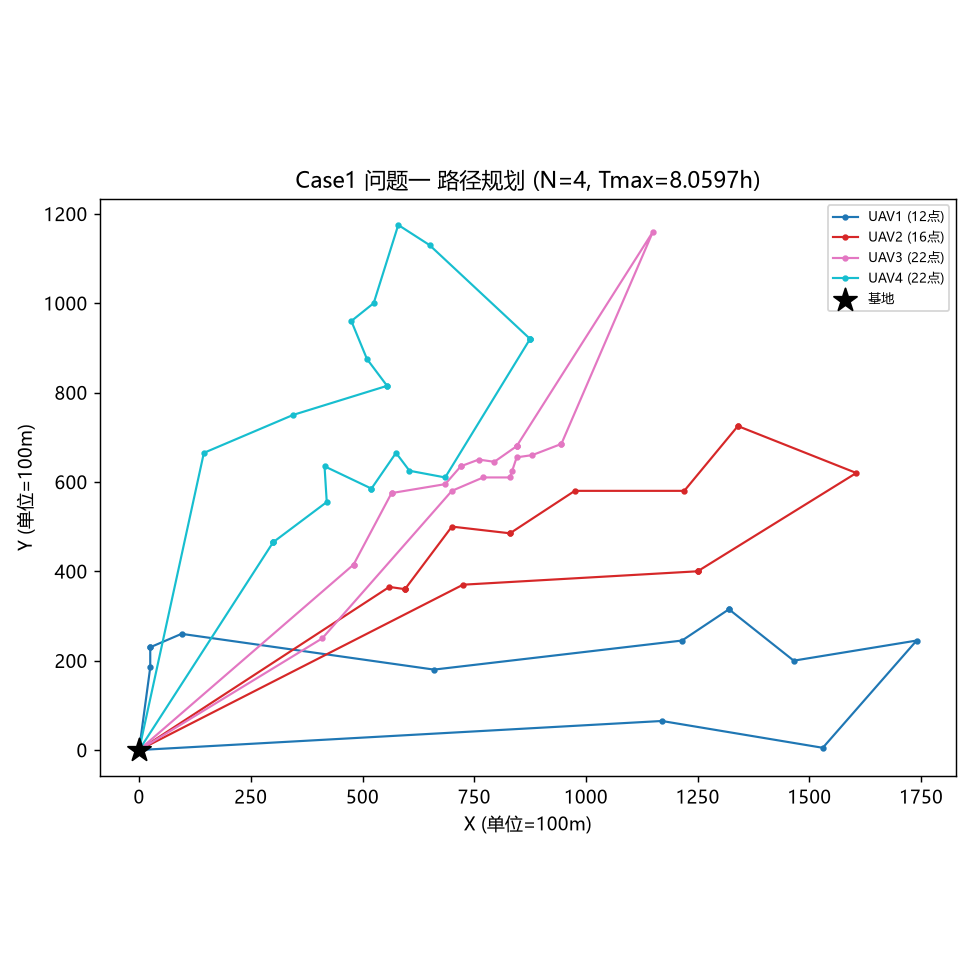
\includegraphics[width=\textwidth]{../figures/Case1_P1.png}
  \end{subfigure}\hfill
  \begin{subfigure}{0.46\textwidth}
    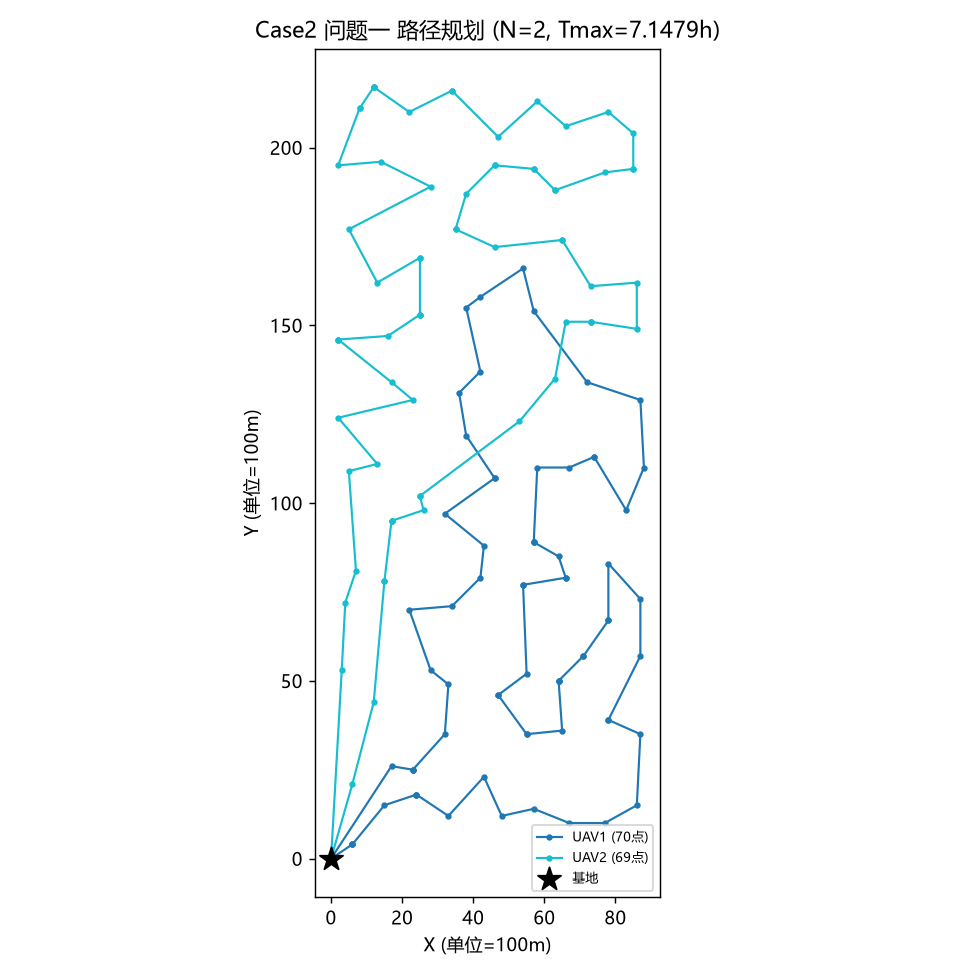
\includegraphics[width=\textwidth]{../figures/Case2_P1.png}
  \end{subfigure}\\[4pt]
  \begin{subfigure}{0.46\textwidth}
    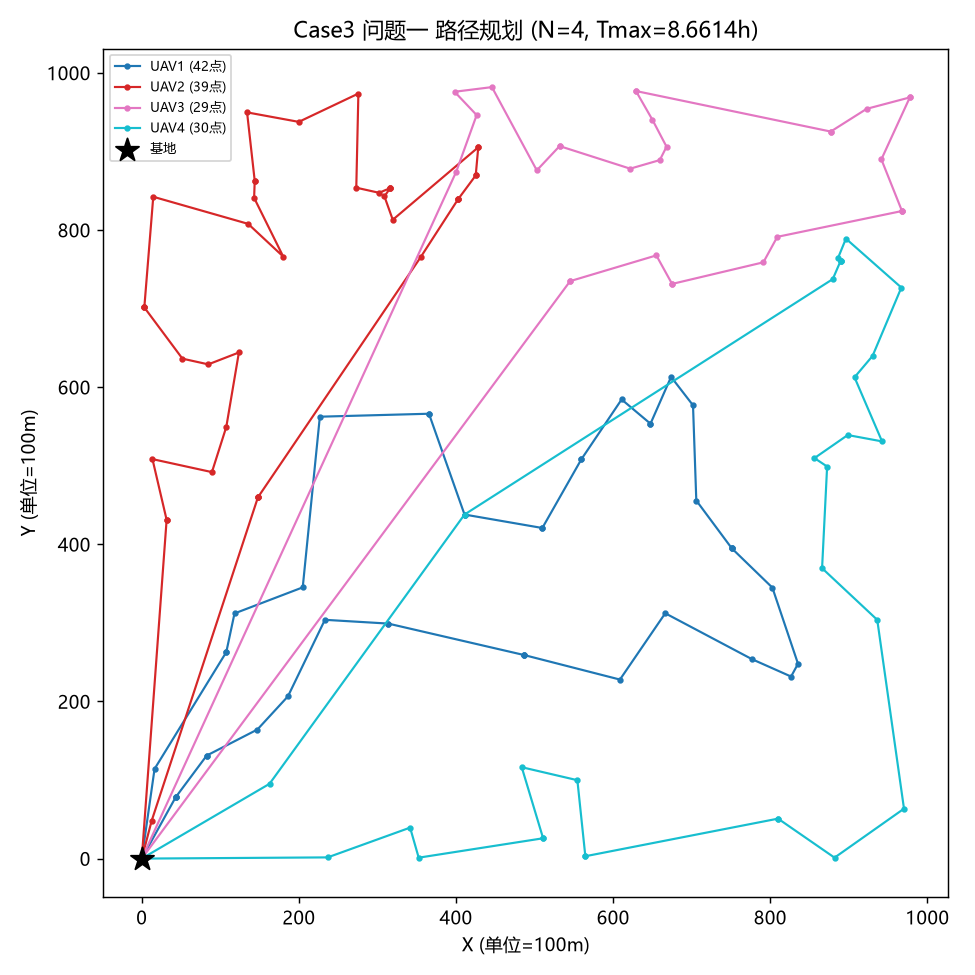
\includegraphics[width=\textwidth]{../figures/Case3_P1.png}
  \end{subfigure}\hfill
  \begin{subfigure}{0.46\textwidth}
    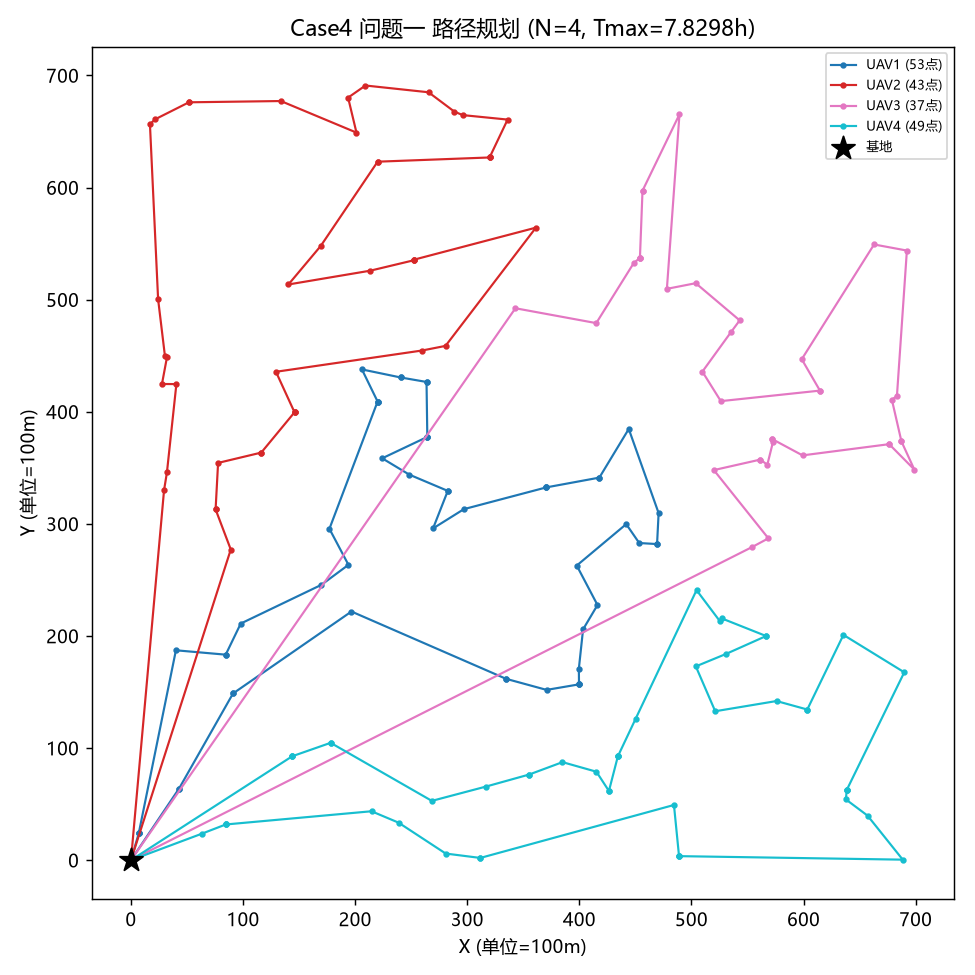
\includegraphics[width=\textwidth]{../figures/Case4_P1.png}
  \end{subfigure}
  \caption{问题一：四个算例的最优巡检路线（$N=N_{\min}$）}
  \label{fig:p1}
\end{figure}

\section{问题二：考虑负载均衡的多机调度模型}

\subsection{字典序优化模型}

问题二要求在总体完成时间尽可能短的同时，使各无人机工作时长尽可能接近。这是一个\textbf{双目标}问题，本文采用\textbf{字典序}处理：第一优先级为 $T_{\max}$，第二优先级为负载差 $\delta=T_{\max}-T_{\min}$，即
\begin{equation}
  \text{lex}\min\ \big(T_{\max},\ \delta\big),
  \label{eq:lex}
\end{equation}
其含义为：在所有 $T_{\max}$ 取到（近似）最优的方案中，进一步选择 $\delta$ 最小的方案。该处理保证不会为了均衡而牺牲总体完成时间。

\subsection{求解方法}

在问题一最优解（或近似最优解）基础上，以式 \eqref{eq:lex} 为接受准则重新执行局部搜索：当候选解的 $(T_{\max},\delta)$ 按字典序小于当前解时接受。搜索过程中若 $T_{\max}$ 增大则立即拒绝，因此所得方案保持问题一的最优（近似）完成时间，同时负载差被进一步压低。

\subsection{结果与分析}

问题二结果见表 \ref{tab:p2}（详细调度方案见 \texttt{result2.xlsx}）。与表 \ref{tab:p1} 对比可见，四个算例的 $T_{\max}$ 保持不变（字典序保证了完成时间不劣化），同时 $\delta$ 均被压缩到 0.03--0.07 h 量级，最大负载差不超过 4.5 min，负载均衡性良好。

\begin{table}[H]
  \centering
  \caption{问题二结果展示表}
  \label{tab:p2}
  \small
  \begin{tabular}{ccccc}
    \toprule
    测试算例 & 无人机数量 $N$ & $T_{\max}$ (h) & $T_{\min}$ (h) & $\delta=|T_{\max}-T_{\min}|$ (h) \\
    \midrule
    Case1 & 4 & 8.0597 & 7.9856 & 0.0742 \\
    Case2 & 2 & 7.1479 & 7.0914 & 0.0565 \\
    Case3 & 4 & 8.6614 & 8.5946 & 0.0668 \\
    Case4 & 4 & 7.8298 & 7.8041 & 0.0257 \\
    \bottomrule
  \end{tabular}
\end{table}

三个问题下各无人机的负载对比见图 \ref{fig:loads}（本图由 AI 工具辅助绘制），可直观看到负载均衡效果。

\begin{figure}[H]
  \centering
  \begin{subfigure}{0.46\textwidth}
    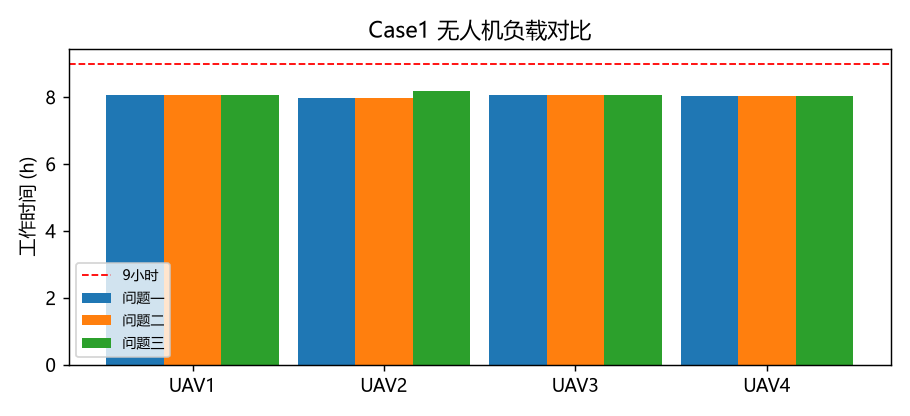
\includegraphics[width=\textwidth]{../figures/Case1_loads.png}
  \end{subfigure}\hfill
  \begin{subfigure}{0.46\textwidth}
    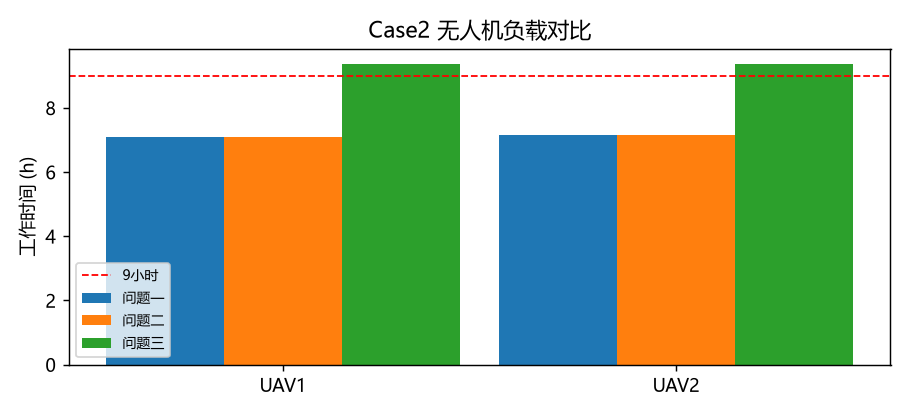
\includegraphics[width=\textwidth]{../figures/Case2_loads.png}
  \end{subfigure}\\[4pt]
  \begin{subfigure}{0.46\textwidth}
    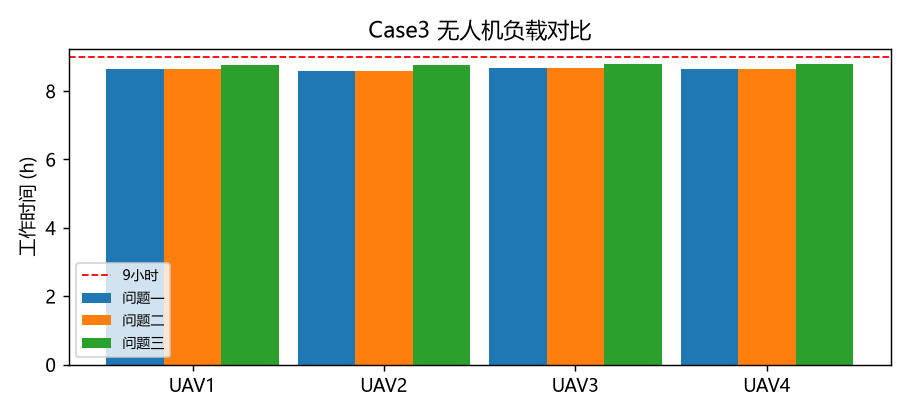
\includegraphics[width=\textwidth]{../figures/Case3_loads.png}
  \end{subfigure}\hfill
  \begin{subfigure}{0.46\textwidth}
    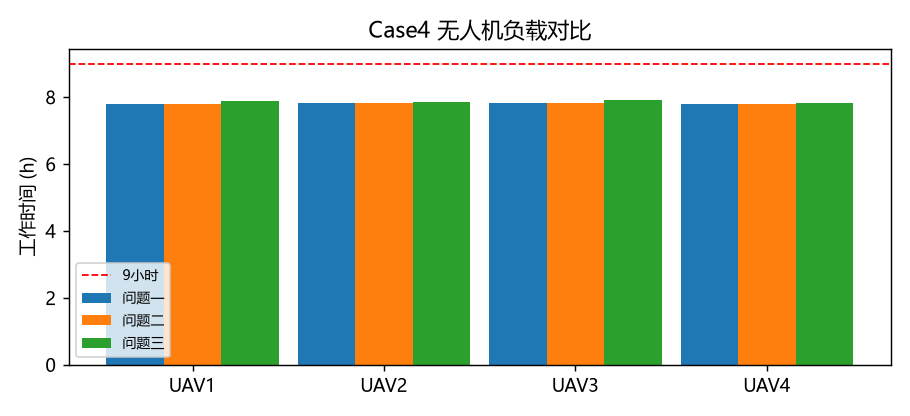
\includegraphics[width=\textwidth]{../figures/Case4_loads.png}
  \end{subfigure}
  \caption{四个算例各无人机在问题一、二、三下的负载对比}
  \label{fig:loads}
\end{figure}

\section{问题三：含时间窗禁飞区的协同巡检模型}

\subsection{禁飞区绕行几何模型}

设航段由点 $a$ 飞往点 $b$，活动禁飞区为圆 $(c,r)$，且 $a,b$ 均在圆外。记
\begin{equation}
  d_u=\|a-c\|,\quad d_v=\|b-c\|,\quad \theta=\angle acb,
\end{equation}
\begin{equation}
  \alpha=\arccos\frac{r}{d_u},\quad \beta=\arccos\frac{r}{d_v},\quad \varphi=\theta-\alpha-\beta.
\end{equation}
当 $\varphi>0$ 时，直线段穿越禁飞区，最短可行绕行路径由两条切线加一段圆弧构成（图 \ref{fig:detour}），其长度为
\begin{equation}
  L=\sqrt{d_u^2-r^2}+\sqrt{d_v^2-r^2}+r\varphi,
\end{equation}
相对直线段的额外距离为 $\Delta=L-\|a-b\|$，额外飞行时间为 $\Delta\cdot 0.1/55$ h；当 $\varphi\le 0$ 时直线段不穿越，无需绕行。

\begin{figure}[H]
  \centering
  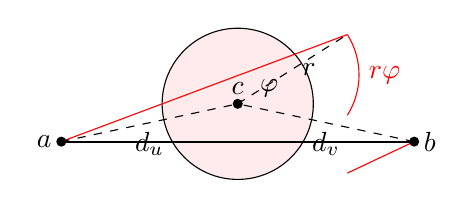
\begin{tikzpicture}[scale=1.6]
    \coordinate (a) at (-1.4,-0.3);
    \coordinate (b) at (1.4,-0.3);
    \coordinate (c) at (0,0);
    \draw[fill=red!8] (c) circle (0.6);
    \draw[thick] (a)--(b);
    \draw[red] (a)--(0.87,0.55);
    \draw[red] (0.87,0.55) arc[start angle=32.3,end angle=-32.3,radius=0.6] node[midway,right]{$r\varphi$};
    \draw[red] (0.87,-0.55)--(b);
    \draw[dashed] (c)--(0.87,0.55) node[midway,right]{$r$};
    \draw[dashed] (a)--(c) node[midway,below]{$d_u$};
    \draw[dashed] (b)--(c) node[midway,below]{$d_v$};
    \fill (a) circle (0.04) node[left]{$a$};
    \fill (b) circle (0.04) node[right]{$b$};
    \fill (c) circle (0.04) node[above]{$c$};
    \draw (0.25,0.12) node{$\varphi$};
  \end{tikzpicture}
  \caption{穿越禁飞区时的切线$+$圆弧绕行路径}
  \label{fig:detour}
\end{figure}

\subsection{时间窗与等待策略}

禁飞区 $z$ 仅在时间窗 $[t_z^0,t_z^1]$ 内活动，因此航段是否绕行取决于\textbf{出发时刻 $t_{\mathrm{dep}}$ 与到达时刻 $t_{\mathrm{arr}}$ 是否与活动窗口重叠}：若 $t_z^0 < t_{\mathrm{arr}}$ 且 $t_z^1 > t_{\mathrm{dep}}$ 且直线段与圆相交，则该航段需绕行。若某巡检点位于活动禁飞区内，则无人机在该点\textbf{等待至 $t_z^1$} 后再执行巡检作业。

\subsection{时间感知的求解算法}

由于路径与时间耦合，本文采用分层求解：

\textbf{Step 1（空间分配）}：忽略禁飞区，用问题二的求解器得到初始的作业分配与路线；

\textbf{Step 2（有效距离矩阵不动点迭代）}：对当前方案按时序仿真，找出需要绕行的航段，将其直线时间替换为绕行时间，得到\textbf{有效距离矩阵} $D_{\mathrm{eff}}$；用 $D_{\mathrm{eff}}$ 重新求解，重复直至绕行航段集合收敛（不动点），从而在规划层面计入绕行代价；

\textbf{Step 3（时间感知重排）}：对每架无人机的作业序列，按``最早可行服务''贪心排序，并用带等待时间的 2-opt 进一步缩短完成时刻，得到满足时间窗约束的实际时刻表；

\textbf{Step 4（轻量再均衡）}：直接评估单作业迁移的完成时间变化，将最长路线的末位作业迁入最短路线，在总完成时间不增加的前提下压缩 $\delta$。

对应程序见附录 B 中 \texttt{zones.py} 与 \texttt{p3b.py}（均由 AI 工具辅助编写）。

\subsection{结果与分析}

问题三结果见表 \ref{tab:p3}（详细调度方案与各点到达/离开时刻见 \texttt{result3.xlsx}）。加入禁飞区后，Case2 因存在大量需绕行或等待的航段，$T_{\max}$ 由 7.15 h 升至 9.38 h，仍接近 9 h 时限且未超限；其余算例最长工作时间仍控制在 8.8 h 以内。四个算例负载差 $\delta$ 均不超过 0.14 h，其中 Case2 两架无人机几乎完全均衡（$\delta=0.003$ h）。

\begin{table}[H]
  \centering
  \caption{问题三结果展示表}
  \label{tab:p3}
  \small
  \begin{tabular}{ccccc}
    \toprule
    测试算例 & 无人机数量 $N$ & $T_{\max}$ (h) & $T_{\min}$ (h) & $\delta=|T_{\max}-T_{\min}|$ (h) \\
    \midrule
    Case1 & 4 & 8.1809 & 8.0425 & 0.1384 \\
    Case2 & 2 & 9.3819 & 9.3788 & 0.0031 \\
    Case3 & 4 & 8.8033 & 8.7546 & 0.0487 \\
    Case4 & 4 & 7.9183 & 7.8143 & 0.1039 \\
    \bottomrule
  \end{tabular}
\end{table}

各算例问题三的路线与禁飞区（红色虚线圈）如图 \ref{fig:p3} 所示（本图由 AI 工具辅助绘制），可看出路线在禁飞区活动时段内成功绕开或等待。

\begin{figure}[H]
  \centering
  \begin{subfigure}{0.46\textwidth}
    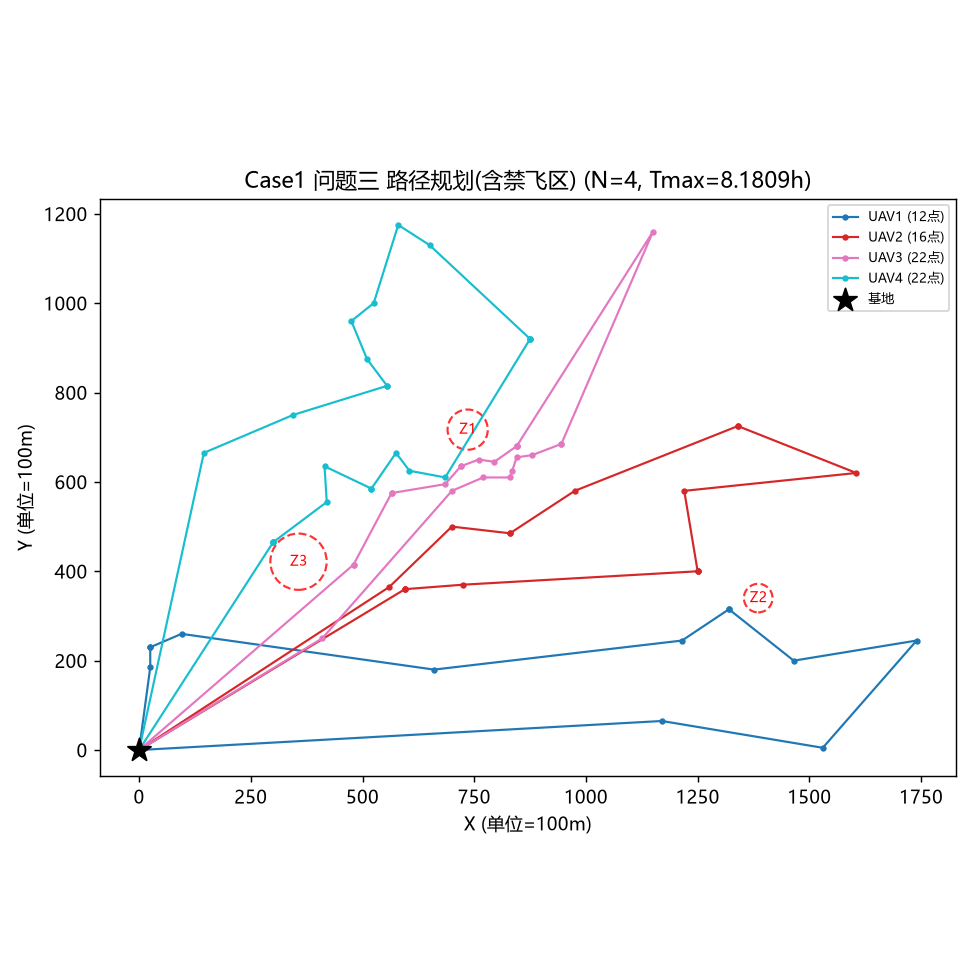
\includegraphics[width=\textwidth]{../figures/Case1_P3.png}
  \end{subfigure}\hfill
  \begin{subfigure}{0.46\textwidth}
    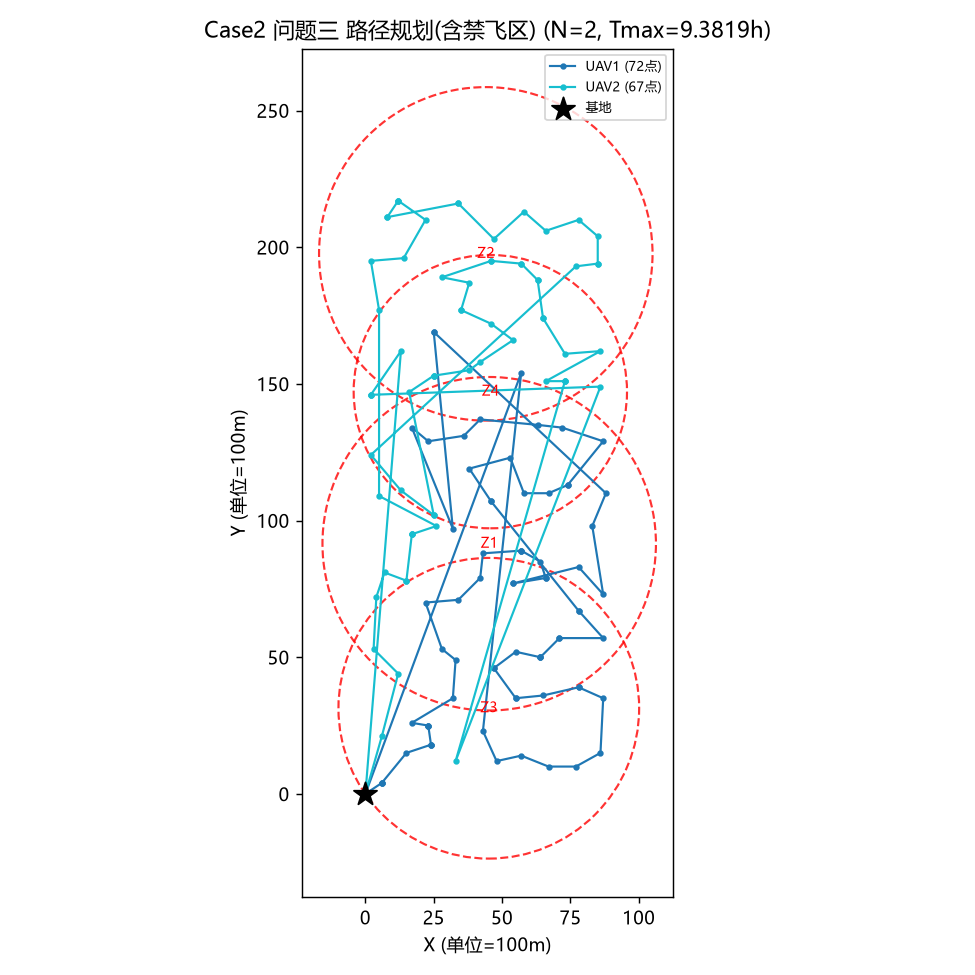
\includegraphics[width=\textwidth]{../figures/Case2_P3.png}
  \end{subfigure}\\[4pt]
  \begin{subfigure}{0.46\textwidth}
    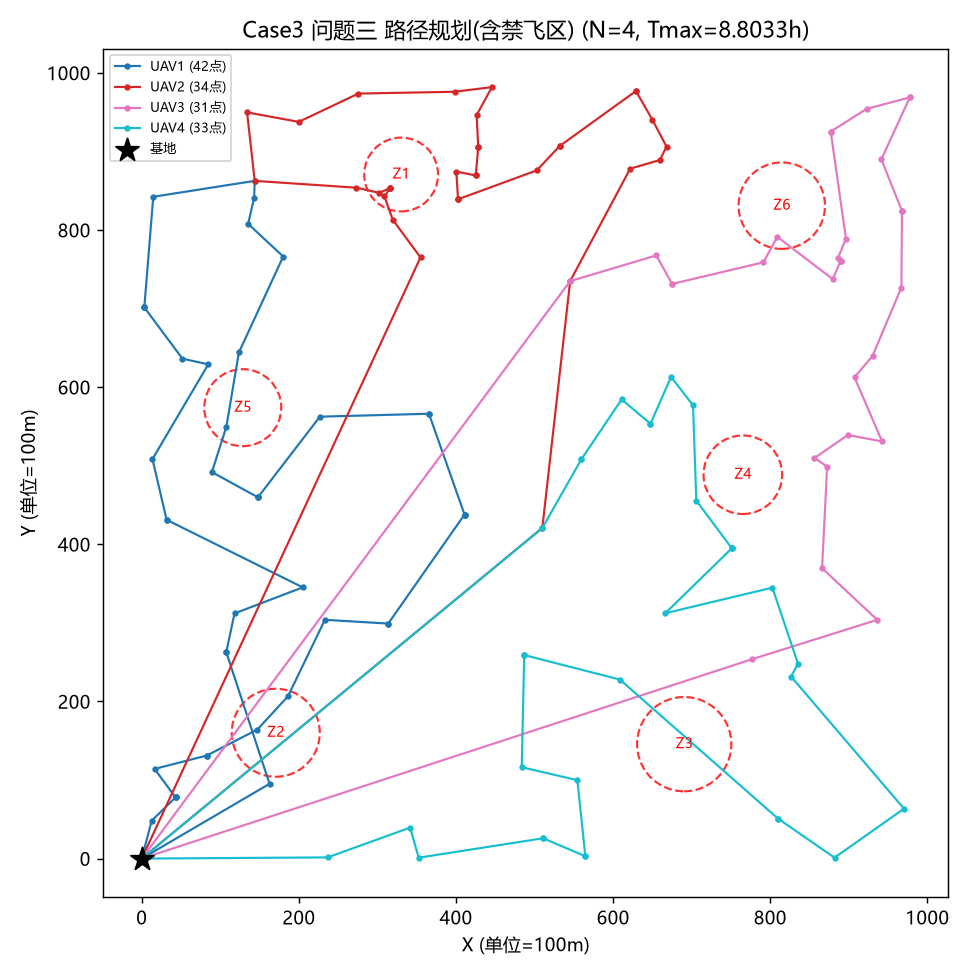
\includegraphics[width=\textwidth]{../figures/Case3_P3.png}
  \end{subfigure}\hfill
  \begin{subfigure}{0.46\textwidth}
    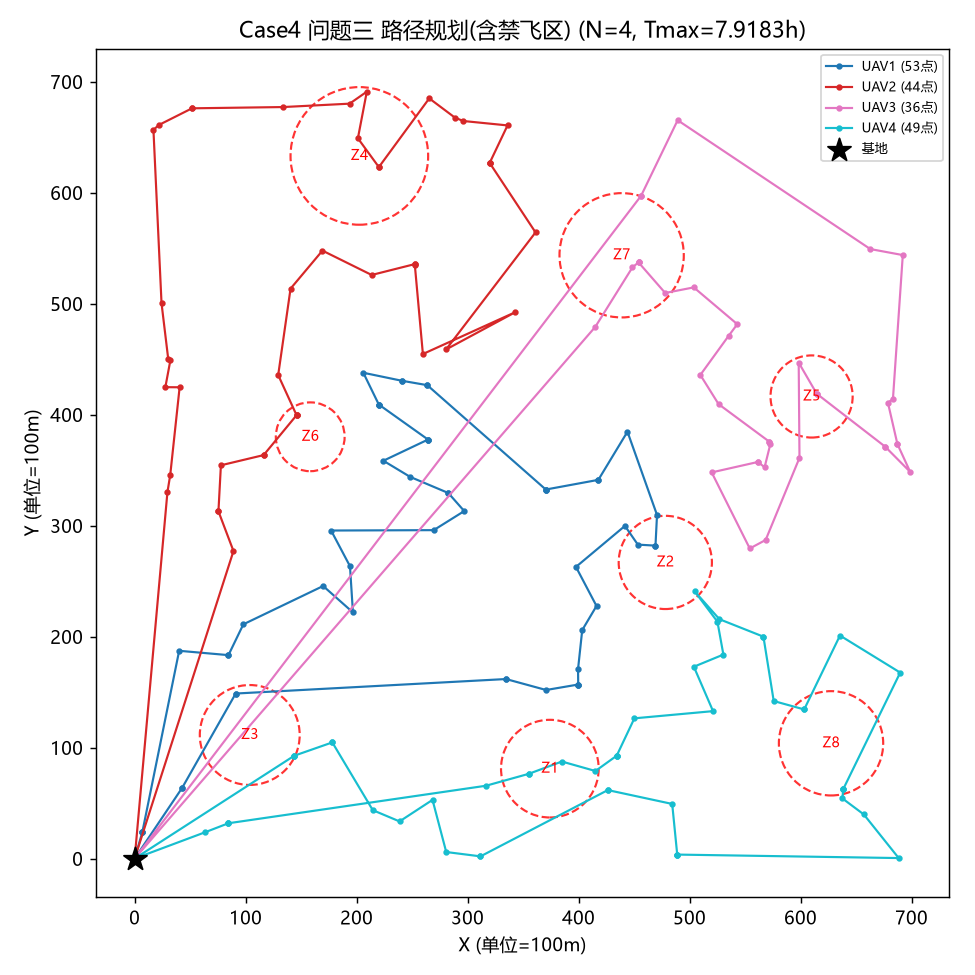
\includegraphics[width=\textwidth]{../figures/Case4_P3.png}
  \end{subfigure}
  \caption{问题三：含禁飞区的最优巡检路线}
  \label{fig:p3}
\end{figure}

\section{模型评价与推广}

\subsection{模型优点}

\begin{enumerate}
  \item 问题一从\textbf{服务时长下界与 MST 飞行时长下界}两个层次给出 $N_{\min}$ 的理论下界，再辅以计算验证，结论严谨、可解释；
  \item 采用\textbf{字典序}处理双目标，严格保证``先优化完成时间、再优化均衡''，避免多目标加权的主观性；
  \item 问题三的``有效距离矩阵不动点迭代 + 时间感知调度''框架，正确处理了路径与时间的耦合，绕行几何模型具有解析形式、计算精确。
\end{enumerate}

\subsection{模型缺点}

\begin{enumerate}
  \item 求解算法属启发式，所得为高质量近似解，无法证明全局最优；
  \item 未考虑无人机续航、充电、起降耗时及空域冲突，与实际部署仍有差距。
\end{enumerate}

\subsection{推广方向}

本文框架可推广至：带容量/续航约束的 VRP、动态禁飞区与在线重规划、三维空域协同与异构无人机机队调度，以及结合强化学习的端到端路径优化等场景。

\section{AI 工具使用说明}

按照《第一届天津市五校数学建模联赛人工智能工具使用规定》，本参赛队声明如下：本文\textbf{核心建模与分析}由参赛队独立完成；文中的\textbf{全部插图与程序代码}在 AI 工具的辅助下生成，正文相应位置已作标注（见图 \ref{fig:p1}、图 \ref{fig:loads}、图 \ref{fig:p3} 及附录 B 说明）。所用 AI 工具已在参考文献 \cite{ai:claude} 中列出，详细使用情况见支撑材料《人工智能工具使用详情.pdf》。

\section{参考文献}

\begin{thebibliography}{9}
\bibitem{dantzig} DANTZIG G B, RAMSER J H. The truck dispatching problem[J]. Management Science, 1959, 6(1): 80-91.
\bibitem{garey} GAREY M R, JOHNSON D S. Computers and intractability: a guide to the theory of NP-completeness[M]. San Francisco: W. H. Freeman, 1979.
\bibitem{lin} LIN S, KERNIGHAN B W. An effective heuristic algorithm for the traveling-salesman problem[J]. Operations Research, 1973, 21(2): 498-516.
\bibitem{kmeans} ARTHUR D, VASSILVITSKII S. k-means++: the advantages of careful seeding[C]//Proceedings of the 18th Annual ACM-SIAM Symposium on Discrete Algorithms. New Orleans: SIAM, 2007: 1027-1035.
\bibitem{toth} TOTH P, VIGO D. The vehicle routing problem[M]. Philadelphia: SIAM, 2002.
\bibitem{ai:claude} Claude, Claude（大语言模型 AI 助手）, Anthropic（Anthropic PBC）, 2026-08-16.
\end{thebibliography}

\clearpage

% ============================================================
%  附录（正文之后，页数不限）
% ============================================================
\appendix
\section*{附录 A\quad 支撑材料文件列表}
\addcontentsline{toc}{section}{附录 A\quad 支撑材料文件列表}

本论文的支撑材料（压缩包）包含以下文件：
\begin{enumerate}
  \item \texttt{result1.xlsx} —— 问题一四个算例的详细调度方案；
  \item \texttt{result2.xlsx} —— 问题二四个算例的详细调度方案；
  \item \texttt{result3.xlsx} —— 问题三四个算例的详细调度方案（含到达/离开时刻）；
  \item \texttt{solve3.py}、\texttt{zones.py}、\texttt{p3b.py}、\texttt{master.py} —— 全部可运行求解程序源代码；
  \item \texttt{figures/} —— 论文中的全部插图（PNG）；
  \item \texttt{人工智能工具使用详情.pdf} —— AI 工具使用详情说明。
\end{enumerate}

\section*{附录 B\quad 源程序代码}
\addcontentsline{toc}{section}{附录 B\quad 源程序代码}

以下为建模所用全部可运行 Python 源程序（由 AI 工具辅助编写），在 Python 3.11 环境（依赖 numpy、scipy、openpyxl、matplotlib）下可直接运行。

\subsection*{B.1\quad solve3.py —— 问题一/二求解器}
\lstinputlisting{../solve3.py}

\subsection*{B.2\quad zones.py —— 禁飞区几何与时序模型}
\lstinputlisting{../zones.py}

\subsection*{B.3\quad p3b.py —— 问题三时间感知求解器}
\lstinputlisting{../p3b.py}

\subsection*{B.4\quad master.py —— 结果输出与绘图总控}
\lstinputlisting{../master.py}

\end{document}
